% !TEX TS-program = lualatex
\documentclass[12pt]{article}
\usepackage{dtj_notas}
\usepackage{sectsty}
\allsectionsfont{\normalfont\sffamily\bfseries}
\usepackage{pgfplots}
\usetikzlibrary{arrows}
\pgfplotsset{samples=300, compat=1.17}
\usepackage{ulem}
\newcommand{\UE}[2]{UE_{\text{#1}}(#2)}
\newtheorem{problem}{Problema}

\title{\sffamily Notas de Unidad 4\\ \textbf{Juegos estáticos con información incompleta}\\ \normalsize Decisiones y Teoría de Juegos}
\author{Emmanuel Alcalá}
\date{\today}

\begin{document}

\maketitle

\hrule

% \begin{summarybox}{Resumen}
% 	\begin{description}
% 		\item[Incertidumbre]

% 	\end{description}
% \end{summarybox}

\section*{Repaso de unidades 1-3}

\paragraph{Utilidad esperada}

\begin{myenum}
	\item ¿Qué diferencia existe entre una cantidad, como el ingreso $ w $, y la utilidad de ese ingreso?
	\item ¿En qué situaciones calcularías la utilidad \textit{esperada}?
	\item ¿Qué actitudes hacia el riesgo existen?
	\item Describe la forma de las funciones de las tres actitudes hacia el riesgo y escribe un ejemplo de una función para cada una de tales actitudes.
	\item Se le ofrecieron a Federico las siguientes cantidades monetarias: $ X = \{0, 100, 400, 10000\} $, y tiene que elegir entre las siguientes dos loterías:
	\[ L_1 = \Biggl\{p(x_1)=\frac{1}{4}, p(x_2)=\frac{1}{4}, p(x_3)=\frac{1}{3}, p(x_4)=\frac{1}{6}\Biggr\} \]
	y
	\[L_2 = \Biggl\{p(x_1)=0, p(x_2)=\frac{1}{4}, p(x_3)=\frac{11}{24}, p(x_4)=\frac{7}{24}\Biggr\} \]
	\begin{myenum}
		\item Representa el anterior problema de decisión \textit{unipersonal} con un árbol.
		\item ¿Cuál de las anteriores loterías le conviene más a Federico? Es decir, ¿qué debería escoger, si es racional?
	\end{myenum}
	\item En el juego del Calamar, los jugadores tienen largas deudas. Deciden entrar a un juego sin saber del todo las consecuencias. Después del primer juego aprenden que el precio por perder es morir. Solo quedan 201 jugadores que votan por abandonarlo, de los cuales 187 regresan. Estos jugadores deciden entrar al juego a sabiendas de que pueden morir, sin embargo, el premio puede que tenga tal incentivo que aún así deciden entrar de nuevo.
	\begin{itemize}
		\item Asumiendo que todos los jugadores tengan la misma probabilidad de ganar, de 1/187, ¿qué actitud hacia el riesgo crees que defina a los jugadores que regresaron?
		\item Supón que ganan 5 si no entran al juego. Supón además que si mueren ganan 0, y si sobreviven ganan 100; la función de utilidad de los jugadores es $ u(x) = x^\alpha $; la probabilidad de vivir es 1/187, y la de morir es su complemento. ¿Para qué valor de $ \alpha $ los jugadores decidirían entrar al juego?
		\item Supón ahora que los jugadores son aversos al riesgo, y tienen un $ \alpha = 0.5 $, pero la probabilidad de sobrevivir es desconocida. ¿Para qué valor de $ p $ decidirían entrar al juego?
	\end{itemize}
\end{myenum}

\paragraph{Juegos estáticos con información completa}

\begin{myenum}
	\item ¿Por qué le llamamos juegos simultáneos?
	\item ¿Cuándo decimos que hemos encontrado un equilibrio en juegos estáticos?
	\item ¿Qué es la eliminacón de estrategias estrictamente dominadas? ¿Por qué son dominadas de forma estricta, y por qué podemos eliminarlas?
	\item ¿Cuál es la diferencia entre una estrategia pura y una estrategia mixta?
	\item ¿Qué es un equilibrio de Nash? (Puedes buscar en inglés \textit{Nash equilibrium}).
	\item En la serie del juego del Calamar, existen juegos que eran jugados más por mujeres que por hombres, y viceversa. Supón el siguiente juego

	\begin{game}{2}{2}[Equipo 1][Equipo 2]
		& Hombres    &   Mujeres    \\
		Hombres    &   (0,0)          &  (-1, 1)   \\
		Mujeres  &   (1, -1)         &  (0,0)
	\end{game}
	\vspace{1em}

	¿Cuál es el equilibrio en estrategias mixtas?
	Nota: estos juegos son de suma cero.

\end{myenum}

\paragraph{Juegos dinámicos con información completa}

\begin{enumerate}
	\setlength{\itemsep}{0pt}
	\setlength{\parskip}{0pt}
	\setlength{\parsep}{0pt}
	\item ¿Cuál es la diferencia entre juegos dinámicos y juegos estáticos?
	\item ¿Qué es un conjunto de información en un juego dinámico?
	\item ¿Por qué podemos jugar un subjuego con información imperfecta como si fuera un juego Simultáneo?
	\item Supón el siguiente juego de negociación. Alberto y Bárbara negocian por el coche de Bárbara. Alberto valora el coche con 5000 dólares, y Bárbara 4500 (él lo valora más porque lo necesita más). Alberto debe ofrecer una cantidad tal que Bárbara esté dispuesta a negociar. Si acepta esa cantidad, la transacción sucede, si no, no ocurre (es decir, se trata de un juego de tipo ultimátum). Para no volverlo un juego bayesiano, asumamos que Alberto conoce el valor de Bárbara por el coche. El juego se puede formular de la siguiente manera (en donde $ x $ es la oferta de Alberto).

	      \begin{figure}[H]
		      \centering
		      \begin{istgame}[font=\scriptsize]
			      \setistgrowdirection{east}
			      \cntmdistance{20mm}{20mm}
			      \cntmAistb{0}[at end,below]{5000}[at end,above]
			      \istrootcntmA(0){Alberto}
			      \istbA[draw=none]
			      \endist
			      % \cntmAistb{0}[at end,below]{5000}[at end,above]
			      \istroot(1)(0-1)<[xshift=-40pt]10>{Bárbara}
			      \istb{Aceptar}[below, yshift=-2pt]{(5000-$x$, x)} \istb{Rechazar}[above, yshift=3pt]{(0, 4500)}
			      \endist
		      \end{istgame}
	      \end{figure}

	      Analiza el juego usando inducción hacia atrá y encuentra la oferta \textit{mínima} que debería hacer Alberto. ¿Qué sería lo mínimo que podría aceptar Bárbara?

	      Nota: Esto ocurre muy a menudo en los depósitos. Cuando rentamos un departamento, el arrendador nos pide un depósito de seguro. Al final del contrato, el arrendador nos puede regresar cualquier cantidad, dado que los contratos usualmente no especifican de forma detallada los términos. Por ejemplo, se puede tomar una fracción del depósito por reparaciones... pero ¿cuáles reparaciones? ¿los inquilinos deben pagarlas? La opción es: toma $\alpha x$ o nos vamos a litigio. Usualmente aceptamos la fracción $ \alpha $. Si depende de nosotros, \textit{nunca} debemos ponernos en una situación en la que solo tengamos la opción de aceptar y no hacer una contraoferta.

\end{enumerate}

\paragraph{Juegos estáticos con información incompleta}

\begin{myenum}
	\item ¿Qué es la información incompleta?
	\item Si vas a tomar una decisión y el resultado depende de lo que alguien más haga, pero desconoces exactamente la decisión del otro agente, ¿qué plan de acción harías?
	\item Supón que el otro agente puede hacer A o puede hacer B, y crees que es igual de probable que haga cualquiera de las dos. Si hace A, tu utilidad sería de 10, y si hace B, tu utilidad sería de 15. ¿Cuál sería tu utilidad esperada?
	\item En los problemas de selección adversa existe información asimétrica. ¿En qué consiste un problema con información asimétrica?
	\item El hecho de que alguien acepte el precio que le das, ¿significa que te conviene? Recuerda el problema de coches usados.
	\item Un asegurador ofrece un plan a un precio Alto (1000) o a precio Bajo (500). Cuesta 400 cubrir a un cliente saludable, y 800 a uno no saludable. Los clientes saludables están dispuestos a pagar 750, mientras que los no saludables 1250. El asegurador desconoce si el jugador es sano o no. El juego (restando las ganancias y los costos) se puede representar así:

	\begin{figure}[H]
		\centering
		\footnotesize{
			\begin{forest} decision tree,for tree={s sep=25pt}
				[Naturaleza, plain content
				[1;{\text{saludable},p},plain content,elo={yshift=4pt},alias=e1i
				[2;Alto,plain content,elo={yshift=4pt}
					[{600,-250};Comprar]
					[{0,0};Re.,elo={yshift=1pt}]
				]
				[2;Bajo,plain content,elo={yshift=4pt}
					[{100,250};Comprar]
					[{0,0};Re.]
				]
				]
				[1;{\text{no saludable},1-p},plain content,elo={yshift=4pt},alias=e1d
				[2;Alto,plain content,elo={yshift=4pt}
					[{200,250};Comprar]
					[{0,0};Re.]
				]
				[2;Bajo,plain content,elo={yshift=4pt}
					[{-300,750};Comprar]
					[{0,0};Re.]
				]
				]
				]
				\draw[dashed,transform canvas={yshift=-6pt}] (e1i) to[right=45] (e1d);
			\end{forest}}
	\end{figure}

	Resuelve con inducción hacia atrás. ¿Cuándo es el precio Alto mejor (es decir, con qué $ p $ de clientes saludables debería ofrecer el precio alto ?

\end{myenum}


\section{Introducción: recapitulación}

Hemos revisado ya 3 situaciones estratégicas donde hemos aplicado un \textbf{concepto de solución} distinto. A continuación se repasan estas situaciones estratégicas y el concepto de solución de equilibrio aplicado.

\begin{summarybox}{}
	\begin{description}
		\item[Juegos {\color{blue!80} estáticos} con información completa] - Juegos simultáneos en donde los jugadores, sus preferencias y los pagos son de \textbf{conocimiento común}. En estos juegos aplicamos el concepto de solución de \textbf{Equilibrio de Nash} en estrategias puras. También, en estos juegos se puede aplicar el concepto de solución de Equilibrio de Nash en estrategias mixtas (aunque se revisó como parte de las soluciones de los juegos dinámicos, cuando existe información imperfecta). Otros conceptos importantes en esta unidad fueron la representación \textbf{normal} del juego y la forma matricial de la representación normal, para dos jugadores, que consiste en un arrego bidimensional.
			\item[Juegos {\color{blue!80}dinámicos} con información completa]- Juegos que suceden en varias etapas, en donde los jugadores van alternando sus acciones. También son llamados juegos secuenciales. Se revisó el concepto de \textbf{racionalidad secuencial}, que implica que en cada \textbf{conjunto de información} en el que el jugador se encuentra, debe maximizar su utilidad. Se revisaron varias estrategias de solución, como la inducción hacia atrás y el concepto de \textbf{Equilibrio de Nash Perfecto en Subjuegos} (ENPS). Otros conceptos importantes en este juego fueron el concepto de \textbf{información imperfecta}.
		\item[Juegos {\color{green!70!black} estáticos} con información {\color{red!70!black}incompleta}] - También llamados juegos bayesianos, en estos juegos simultáneos, las preferencias de los jugadores o sus pagos no son de conocimiento común. Denotamos al conjunto de información que es \textbf{privada} para un jugador (o para todos) por \textbf{el tipo} de un jugador. En estos juegos requerimos que el jugador desinformado tenga creencias, o conjeturas, sobre la información que desconoce (el tipo). Esas creencias son representadas como una distribución de probabilidad sobre los tipos. Introdujimos el concepto de solución de \textbf{Equilibrio de Nash Bayesiano}, o ENB.
	\end{description}
\end{summarybox}

En esta unidad centraremos la atención en un cuarto tipo de juegos, los juegos dinámicos con información incompleta.


\subsection{Conceptos de solución}

\begin{enumerate}
	\setlength{\itemsep}{0pt}
	\setlength{\parskip}{0pt}
	\setlength{\parsep}{0pt}
	\item Un \textbf{concepto de solución} es una regla formal de predicción sobre cómo será jugado un juego.

	\item Las predicciones son soluciones que describen las estrategias que los jugadores adoptarán, y por lo tanto, el resultado del juego.

	\item Los conceptos de \textbf{equilibrio} revisados son una clase de esos conceptos de solución.
\end{enumerate}

Normalmente, tener más de una solución no es algo deseable, a menos de que se desee justamente evaluar de qué soluciones se dispone. Si se quiere intervenir en algo para que el juego se desarrolle en el sentido que un jugador desea, entonces es preferible tener una solución única. En ese caso, se han aplicado refinamientos.

Los refinamientos que hemos revisado se pueden resumir en la siguiente table

\begin{table}
	\centering
	\begin{game}{2}{2}[Información][Desarollo temporal]
		& Simultáneo    &   Secuencial    \\
		completa    &   EN          &  ENPS   \\
		incompleta  &   ENB         &  EBP
	\end{game}
	\caption{Conceptos de solución y refinamientos.}
\end{table}

\begin{myenum}
	\item Si en un juego dinámico analizamos cada subjuego por separado, llegaríamos a múltiples equilibrios, pero al aplicar inducción hacia atrás eliminamos las estrategias dominadas y, asumiendo racionalidad, tenemos solo una ruta de equilibrio para todos los jugadores, lo que nos asegura ganancias únicas.
	\item La idea es crear un perfil de estrategias que se pueda usar un lugador para llegar al resultado deseado (al resultado de la solución del equilibrio).
	\item Si creamos un perfil para una empresa, debería ser posible que un CEO nuevo tomase el perfil en cualquier punto del juego y tendría qué saber qué hacer. Por eso llamamos a ese perfil ENPS un plan de acción completo.
	\item En cada subjuego de un juego dinámico encontramos solución óptimas (racionalidad secuencial).
\end{myenum}

De nuevo: un equilibrio se logra si ningún jugador tene un incentivo extra para desviarse de una estrategia. En toda situación estratégica debemos identificar si existe dicho incentivo.

En juegos dinámicos con información completa, las estrategias forman un equilibrio en el juego completo (el ENPS), pero también forman un equilibrio de Nash en cada subjuego.


Como vimos en la pasada unidad, cuando existe información privada, los jugadores se representan dicha información (que llamamos \textit{tipos}) como una distribución de probabilidad sobre los tipos.

En un juego dinámico, esos tipos pueden dar lugar a muchos subjuegos (cada uno iniciado con la probabilidad de algún tipo), debido a que habrá muchos conjuntos de información.


% \begin{mybox}[colback=red!20]{Nota:}
% 	Antes de comenzar, necesitamos saber \textit{qué nos hace falta} para poder analizar juegos dinámicos con información incompleta.
% \end{mybox}


% \subsection{Juego de Stackelberg}

% En la competencia de Stackelberg una empresa líder, llamémosla E1 decide una cantidad a producir $ q_1 $.

% Supongamos que E1 puede tener costo marginal bajo o costo marginal alto ($ c_B $ o m,$ c_A $, respectivamente). El costo de E2 es conocido. E1 escoge $ q_1=4 $ ó $ q_1=8 $.

% De nuevo haremos la simplificación de que es la Naturaleza (N) quien elige qué tipo de costo tendrá E1. Recordar que el jugador N se ignora posteriormente.

% \textbf{Crucial:} E2 \textit{observa} la cantidad elegida de por E1, pero \textit{no observa} el tipo de E1 (es decir, no observa si el costo fue alto o bajo). Por lo tanto, si E1 eligió $ q_1=4 $, esto puede ocurrir bajo costo bajo $ c_B $ o bajo costo alto $ c_A $.

% En el árbol, el conjunto de información cuando E2 tome su decisión son dos nodos con diferente predecesor: cuando E1 tiene costo bajo y cuando E1 tiene costo alto. Lo mismo ocurre si E1 elige $ q_1=8 $.

% \begin{figure}[H]
% 	\centering
% 	\footnotesize{
% 		\begin{forest} decision tree,for tree={s sep=25pt, l sep=20pt}
% 			[N,plain content,elo={yshift=4pt}
% 			[E1;c_B,plain content,elo={yshift=4pt},alias=c2i
% 			[E2;{q_1=4},plain content,elo={yshift=4pt},alias=E20
% 			[{5,5}; {q_2=4},elo={xshift=-3pt}]
% 			[{3,7}; {q_2=8}]
% 			]
% 			[E2;{q_1=8},plain content,elo={yshift=4pt},alias=E21
% 			[{7,7}; {q_2=4}]
% 			[{10,12}; {q_2=8}]
% 			]
% 			]
% 			[E1;c_A,plain content,elo={yshift=4pt},alias=c2d
% 			[E2;{q_1=4},plain content,elo={yshift=4pt},alias=E22
% 			[{2,5}; {q_2=4}]
% 			[{1,6}; {q_2=8}]
% 			]
% 			[E2;{q_1=8},plain content,elo={yshift=4pt},alias=E23
% 			[{0,12}; {q_2=4}]
% 			[{5,5}; {q_2=8}]
% 			]
% 			]
% 			]
% 			\draw[dashed,transform canvas={yshift=-10pt}] (E20) to[out=15, in=165] (E22);
% 			\draw[dashed,transform canvas={yshift=-9pt}] (E21) to[out=15, in=165] (E23);
% 			\node[draw=white, fill=white,right=9pt of c2i] at (c2i) {$ [\theta] $};
% 			\node[draw=white, fill=white,left=9pt of c2d] at (c2d) {$ [1-\theta] $};
% 		\end{forest}}
% \end{figure}

% El perfil de estrategias se debe asignar por jugador y por tipo. Por cada nodo de decisión, una estrategias mapea a una acción. Para E1

% \begin{align*}
% 	S_1^B = \{4, 8\} \\
% 	S_1^A = \{4, 8\}
% \end{align*}

% Tiene las mismas estrategias pero porque así lo definimos. Podría tener estrategias diferentes.

% Para E2 tenemos 4 nodos, por lo que necesitamos 4 acciones

% \[
% 	S_2 =	\{44, 48, 84, 88\}
% \]

% El perfil del jugador 2 es una acción por cada infoset: $ S_2 = S_2^BS_2^A $. En el primer caso, 44 significa que E2 escogerá 4 en ambos conjuntos de información; 48 significa que en el primero escogerá 4 y en el segundo 8, 84 que escogerá 8 en el primero y 4 en el segundo y 88 que escogerá 8 en ambos. La representación se hace así por la razón de que la E2 no sabe en qué nodo se encuentra.



% Algunos autores suelen representar los juegos dinámicos como juegos estratégicos (normales), pero esta representación hace que la información temporal se pierda. El juego se puede representar en forma normal como

% \begin{figure}[H]
% 	\centering
% 	\begin{tikzpicture}
% 		\node(0)[circle,draw,inner sep=1.5,fill=black,label=above:$N$]{}
% 		[grow'=south,sibling distance=8cm,transform canvas={xshift = 0.6cm}]
% 		child{edge from parent node[right=4pt]{$c_A$}}
% 		child{edge from parent node[left=6pt]{$c_B$}}
% 		;
% 		\node[anchor=north]at(0-1){
% 			\begin{game}24[$E1$][$E2$]
% 				& 44   & 48  & 84   & 88 \\
% 				4 & 2,5  & 2,5 & 1,6  & 1,6 \\
% 				8 & 0,12 & 5,5 & 0,12 & 5,5
% 			\end{game}
% 		};
% 		\node[anchor=north]at(0-2){
% 			\begin{game}24[$E1$][$E2$]
% 				& 44 & 48 & 84 & 88 \\
% 				4 & 5,5 & 5,5 & 3,7 & 3,7\\
% 				8 & 7,7 & 10,12  & 7,7 & 10,12
% 			\end{game}
% 		};

% 	\end{tikzpicture}
% \end{figure}

% La matriz izquierda solo tiene que ver con los costos bajos. El primer número de cada estrategia indica el infoset. Cuando E1 escoge 4, y si E2 escoge 4 (que sucede dos veces: 44 y 48), su ganancia es (5,5). Si E1 escoge 8 y E2 escoge 4 (segunda acción), ganan 7,7, pero si E2 escoge 8 (segunda acción), ganan 10,12.

% Notar que la primera acción en el par 44 corresponde a la respuesta de E1 a la primera acción de E1.

% ¿Cuál es el equilibrio en este juego?

% Podemos evaluar cada una de las estrategias de cada jugador.

% \begin{figure}[H]
% 	\centering
% 	\begin{tikzpicture}
% 		\node(0)[circle,draw,inner sep=1.5,fill=black,label=above:$N$]{}
% 		[grow'=south,sibling distance=8cm,transform canvas={xshift = 0.6cm}]
% 		child{edge from parent node[right=4pt]{$c_A$}}
% 		child{edge from parent node[left=6pt]{$c_B$}}
% 		;
% 		\node[anchor=north]at(0-1){
% 			\begin{game}24[$E1$][$E2$]
% 				& 44   & 48  & 84   & 88 \\
% 				4 & (2),5  & 2,5 & (1),6  & 1,6 \\
% 				8 & 0,12 & (5),5 & 0,12 & (5),5
% 			\end{game}
% 		};
% 		\node[anchor=north]at(0-2){
% 			\begin{game}24[$E1$][$E2$]
% 				& 44 & 48 & 84 & 88 \\
% 				4 & 5,5 & 5,5 & 3,7 & 3,7\\
% 				8 & (7),7 & (10),12  & (7),7 & (10),12
% 			\end{game}
% 		};

% 	\end{tikzpicture}
% \end{figure}

% Podemos hacernos la pregunta: si el E1 juega (8,4) (para sus tipos bajo y alto), y el jugador E2 juega 44, ¿es este un EBN? Es decir, ¿44 es una MR de E2 a (8,4) de E1?

% \[
% 	UE_2(8,4; 44)=7q + 5(1-q)	= 5 + 2q
% \]

% Podemos compararla con otra estrategia de E2

% \[
% 	UE_2(8,4; 48)=12q + 5(1-q)= 5 + 7q
% \]

% Podemos ver que para cualquier valor de $ q $, 48 sería mejor estrategia. El perfil de estrategias $ s^*=(8,4; 44) $ no es un ENB. Podemos repetir el proceso de forma interativa para todas las estrategias. Deberíamos encontrar el equilibrio, pero \textit{sería un ENB}. ¿Nos sirve esto?

% Veamos otro problema.

% \begin{figure}[H]
% 	\centering
% 	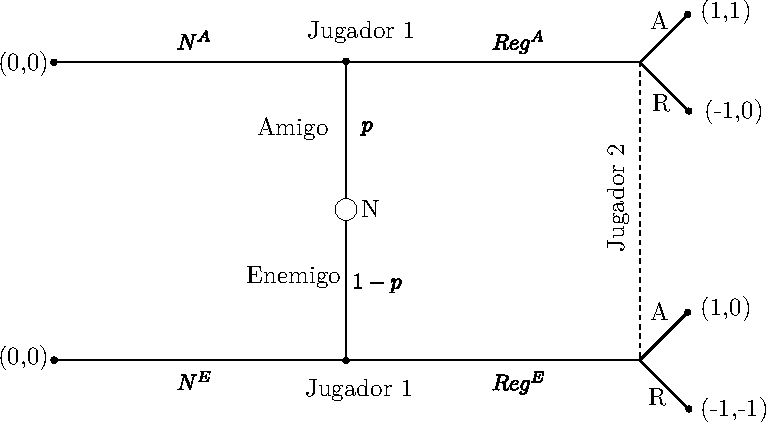
\includegraphics{gift_game.pdf}
% \end{figure}

% El jugador 1 decide darle un regalo ($ Reg $) al jugador 2. El jugador 1 está privadamente informado acerca de si es un jugador amistoso ($ A $) o enemistoso ($ E $). El jugador 2 no lo sabe, y debe decidir si Aceptar (A) o Rechazar (R).

% Las estrategias del jugador 1 son $ S_2 = S^FS^E = \{Reg^A Reg^E, Reg^A N^E, N^A Reg^E ,N^A N^E \} $, y las del jugador 2 $S_2= \{A, R\} $.

% \begin{center}
% 	\begin{game}42[$j1$][$j2$]
% 		& A & R  \\
% 		$Reg^A Reg^E$ & 1, $ p $ & -1, $ p - 1$ \\
% 		$Reg^A N^E$ & $ p,p $  & $ -p, 0 $    \\
% 		$N^A Reg^E$ 		& $1-p,0$  & $ p-1, p-1 $ \\
% 		$N^A N^E$ 		& 0,0			 & 0,0
% 	\end{game}

% \end{center}


% Las ganancias fueron computadas ya como utilidades esperadas. Por ejemplo,

% \[
% 	UE_1(Reg^A Reg^E; A) = \underbrace{1p}_{\text{1 amigable regala, 2 acepta}}+\underbrace{(1-p)1}_{\text{1 no amigable regala, 2 acepta}}=1
% \]

% \[
% 	UE_2(Reg^A Reg^E; A) = \underbrace{1p}_{\text{1 amigable regala, 2 acepta}}+\underbrace{(1-p)0}_{\text{1 no amigable regala, 2 acepta}}=p
% \]

% \[
% 	UE_1(Reg^A N^E; A) = \underbrace{1p}_{\text{1 amigable regala, 2 acepta}}+\underbrace{(1-p)0}_{\text{1 no amigable N, 2 acepta}}=p
% \]

% \[
% 	UE_1(Reg^A N^E; A) = \underbrace{1p}_{\text{1 amigable regala, 2 acepta}}+\underbrace{(1-p)0}_{\text{1 no amigable N, 2 acepta}}=p
% \]

% Y así por el estilo. Si tratamos de encontrar el EN en este juego con el método de 3 pasos, nos quedaría (asumiendo $ 0<p<1 $). \footnote{
% 	Para cada columna, evaluar a j1, para cada fila, evaluar a j2.
% }.

% Si j2 elige A, la mejor respuesta de j1 es $ Reg^A Reg^E $ (obtiene 1), pero si j2 elige R, la mejor respuesta de j1 es $ N^A N^E $, y obtiene 0.

% \begin{center}
% 	\begin{game}42[$j1$][$j2$]
% 		& A & R  \\
% 		$Reg^A Reg^E$ & (1), $ (p) $ & -1, $ p - 1$ \\
% 		$Reg^A N^E$ & $ p,(p) $  & $ -p, 0 $    \\
% 		$N^A Reg^E$ 		& $1-p,(0)$  & $ p-1, p-1 $ \\
% 		$N^A N^E$ 		& 0,(0)		 & (0),(0)
% 	\end{game}

% \end{center}

% Tenemos dos equilibrios: $ (Reg^A Reg^E, A) $ y $( N^A N^E, R )$. Pero... ¿$( N^A N^E, R )$ es racional para el jugador 2? No. Revisar la parte derecha del árbol. Independientemente del tipo del jugador 1, j2 siempre acepta regalos, pero el equilibrio $( N^A N^E, R )$ no incorpora esa preferencia. El infoset del jugador 2 nunca es alcanzado en ese equilibrio.


% Tanto en estos juegos como en los revisados en la unidad 2, debemos exigirle a los jugadores ser \textit{secuencialmente racionales}. En la unidad 2 encontramos que la racionalidad secuencial nos llevaba al concepto de ENPS. Pero ¿tenemos subjuegos en este juego? ¿Cuántos subjuegos tenemos? Solo tenemos un subjuego. Cualquier solución a este juego no nos diría qué haría cada jugador en cada etapa del juego.


% \begin{mybox}[colback=red!15, coltitle=black]{Nota: racionalidad secuencial y equlibrio bayesiano perfecto}

% 	Los jugadores  mazimizan sus ganancias \textit{en cada infoset} en el que se encuentran. Esto debería ser suficiente para analizar un juego dinámico, pero en el juego que presentamos no es así, porque solo existe un subjuego (el propio juego).

% 	Necesitamos \textit{aislar} cada conjunto de información para analizarlo y verificar qué estrategias en ese infoset son racionales.

% 	Eso es lo que hace el equilibrio bayesiano perfecto (EBP).

% \end{mybox}

\section{Equilibrio Bayesiano Perfecto, EBP}


En el anterior juego, debemos poder aislar al jugador 2 en cada uno de sus infosets incluso si no inicia un subjuego. Para esto, requeriremos del jugador 2 que tenga creencias en su infoset.

\begin{mybox}{Requerimiento 1}
	En cada infoset, el jugador que mueve debe tener una creencia (o conjetura) respecto en cual nodo se encuentra o qué nodo ha sido alcanzado. Para un infoset no unitario, una creencia es una distribución de probabilidad sobre los nodos en el infoset; para un infoset unitario, se asigna probabilidad de 1 al único nodo.
\end{mybox}

Sea $ H_i $ el conjunto de todos infosets del juego del jugador i, con $ h_i \in H_i $ denotando uno de tales conjuntos de información en una etapa. Para cada conjunto $ h_i \in H_i $ y cada nodo $ x_k \in h_i $, $ \phi(x_k) \in [0, 1] $ es la probabilidad que el jugador $ i $ que mueve en $ h_i $ asigna al nodo $ x_k $, en donde $ \sum_{x\in h} \phi(x)=1$ par todo $ h \in H $.

Por ejemplo, el jugador 2 en el juego del regalo tiene un solo conjunto de información $ h_2 = \{x_a, x_b\} $ (en donde $ x_a $ es el nodo \textit{arriba} y $ x_b $ es el nodo \textit{abajo}). El \textbf{Requerimiento 1} exige que el jugador 2 asigna una probabilidad $ \phi(x_a) = \phi $ y $ \phi(x_b) = 1-\phi $.

\begin{mybox}{Requerimiento 2}

	Dadas sus creencias (o conjeturas), las estrategias de los jugadores deben ser \textit{sucesivamente racionales}. En cada infoset $ h $, la acción del jugador al que le toca mover \textbf{y} su estrategia subsiguiente deben ser óptimas, dada la conjetura del jugador en ese infoset y las subsiguientes estrategias de los \textit{demás jugadores}. Por estrategia subsiguiente nos referimos a un plan de acción que cubre cada contingencia que podría suceder luego de haber alcanzado el infoset $ h $.

\end{mybox}

\begin{figure}[H]
	\centering
	\footnotesize{
		\begin{forest} decision tree,for tree={s sep=20pt, l sep=25pt,anchor=center}
			[1,plain content,elo={yshift=4pt}
			[{{\scriptsize[\phi]}, 2};L,plain content,elo={yshift=4pt},alias=c2i
			[{2,1}; {u}]
			[{0,0}; {D}]
			]
			[{2, {\scriptsize[1-\phi]}};M,plain content,elo={yshift=4pt},alias=c2d
			[{0,2}; u,elo={yshift=4pt}]
			[{0,1}; D,elo={yshift=4pt}]
			]
			[{1,3}; R, elo={yshift=4pt}]
			]
			\draw[dashed,transform canvas={yshift=-10pt}] (c2i) to[out=15, in=165] (c2d);
			% \draw[dashed,transform canvas={yshift=-9pt}] (E21) to[out=15, in=165] (E23);
			% \node[draw=white, fill=white,left=10pt of c2i] at (c2i) {\scriptsize$ [\theta] $};
			% \node[draw=white, left=5pt of c2d] at (c2d) {\scriptsize$ [1-\theta] $};
		\end{forest}}
\end{figure}

La representación estratégica del juego se muestra en la siguiente tabla, en donde se representa entre paréntesis las estrategias que son MR.

\begin{center}
	\begin{game}32[$j1$][$j2$]
		& U & D  \\
		L & (2),(1) & 0,0 \\
		M & 0,(2) & 0,1 \\
		R & 1,3 & (1),(3)
	\end{game}
\end{center}

Tenemos dos equilibrios, pero uno de ellos no es creíble. El jugador 2 solo juega D si se alcanza su nodo de decisición, pero en ese caso (R,D) prefiere U.

Si aplicamos el \textbf{Requerimiento 2}, entonces podríamos comenzar a resolver el juego para el jugador 2, dadas sus estrategias U y D.

\begin{align*}
	UE_2(D)=\phi(0) + (1-\phi)1 = 1-\phi \\
	UE_2(U) = \phi(1) + 2(1-\phi) = 2-\phi
\end{align*}

Se puede ver claramente que U es dominante, ya que $\UE{2}{U} > \UE{2}{D}$. El juego ahora estaría reducido a solo dos opciones: L y R (con j2 jugando U).

\begin{figure}[H]
	\centering
	\footnotesize{
		\begin{forest} decision tree,for tree={s sep=20pt, l sep=25pt,anchor=center}
			[1,plain content,elo={yshift=4pt}
			[{{\scriptsize[\phi]=0}, 2};L,plain content,elo={yshift=4pt},alias=c2i
			[{2,1}; {u}]
			[{0,0}; {D}]
			]
			[{2, {\scriptsize[1-\phi]=1}};M,plain content,elo={yshift=4pt},alias=c2d
			[{0,2}; u,elo={yshift=4pt}]
			[{0,1}; D,elo={yshift=4pt}]
			]
			[{1,3}; R, elo={yshift=4pt}]
			]
			\draw[dashed,transform canvas={yshift=-10pt}] (c2i) to[out=15, in=165] (c2d);
		\end{forest}}
\end{figure}

Supongamos que $ \phi = 0 $, y ahora tenemos la estrategia $ (L, U; \phi = 0) $. ¿Cómo interpretarlo? $ \phi=0 $ es una creencia que solo se aplica una vez que se ha alcanzado el nodo del infoset del jugador 2, no antes. Ser secuencialmente racional implica estar en ese nodo, aplicar la creencia para el resto de nodos subsiguientes, no predecesores.

No importa aquí si esta creencia es correcta o incorrecta, sino que se comporte racionalmente y sea consistente con dicha creencia. En particular, esta creencia implica que el jugador 2 se encuentra en el nodo derecho ($ x_3 $).

Ahora bien, ¿la conjetura misma es razonable? Para repsonder, debemos imponer un requisito sobre las conjeturas, pero antes recordemos la distinción entre conjuntos de información.

\begin{mybox}{Definición}
	\begin{defi}
		Para un equilibrio dado en un juego con forma extensiva, un infoset está en la trayectoria del equilibrio si se alcanza con probabilidad positiva, y fuera de la trayectoria si la probabilidad de que se alcance es 0.

		\textit{Cuando el juego se juega según las estrategias en equilibrio}. Notar que se presupone que se encontró un equilibrio, pero no necesariamente un EBP.
	\end{defi}

\end{mybox}

Si vamos a jugar un perfil de estrategias en equilibrio (sea EBP o no), algunos infoset se alcanzan o no se alcanzan.

Considerar el siguientes conjunto de estrategias (por el momento no nos preocupamos si son estrategias en equilibrio). ¿El infoset del jugador 2 está en la ruta del equilibrio?

\begin{myenum}
	\item $\biggl( \frac{1}{2}L, \frac{1}{2}R, U; \phi \biggr)$: sí, es alcanzado cuando toma L.
	\item $( R, U; \phi )$: no, nunca es alcanzado. Notar que aún así, se incluye U como una estrategia óptima \textit{dado} que el conjunto de información se alcanzara.
	\item $ (L, D; \phi) $. L se juega con probabilidad 1, por lo que sí se encuentra en la ruta.
\end{myenum}

Ahora imponemos el siguiente requisito a las creencias

\begin{mybox}{Requerimiento 3}

	En los infosets que están en la ruta del equilibrio, las creencias deben ser determinadas por la regla de Bayes y las estrategias en equilibrio de los jugadores.

\end{mybox}

Consideremos $\biggl( \frac{1}{2}L, \frac{1}{2}R, U; \phi \biggr)$.

¿Para qué valores de $ \phi $ las estrategias y las creencias del jugador 2 son consistentes?

Notar que la probabilidad de estar en nodo izquierdo, $ \phi $, es condicional a L, que sucede con probabilidad 1/2.

\begin{align*}
	\phi = \frac{ \frac{1}{2} }{\frac{1}{2} + 0}
\end{align*}

En el denominador, la probabilidad de alcanzar el conjunto de información donde el jugador 2 decide. Eso sería la $ \sigma(L) + \sigma(M) = 1/2 + 0 $.

Por lo tanto $ \phi = 1$. Esto es consistente: dado que el jugador 2 alcanzara dicho nodo de información, \textit{no pudo} haberlo alcanzado porque el jugador 1 jugó M.

Más aún: si $ \phi < 1$, ello implicaría que $ \sigma(M) \neq 0 $, y por lo tanto $\biggl( \frac{1}{2}L, \frac{1}{2}R, U; \phi \biggr)$ no sería consistente. Por lo tanto, $\biggl( \frac{1}{2}L, \frac{1}{2}R, U; \phi \biggr)$ satisface R3 si y solo sí $ \phi = 1 $.

Supongamos que tenemos el equilibrio $\biggl( \frac{1}{3}L, \frac{1}{3}M, \frac{1}{3}R, U; \phi \biggr)$

¿Qué valor de $ \phi $ satisface R3?

\[
	\phi = \frac{\frac{1}{3}}{\frac{1}{3} + \frac{1}{3}} = \frac{1}{2}
\]

¿Qué hay del equilibrio $( R, U; \phi )$? Tanto L como M suceden con probabilidad de 0. R3 no nos dice qué hacer con los nodos que se encuentran fuera del equilibrio.

\begin{mybox}{Requerimiento 4}
	En infosets que estén fuera de la ruta del equilibrio, las creencias son determinadas por la regla de Bayes y las estrategias de los jugadores \textit{siempre que sea posible}.

\end{mybox}

\begin{mybox}{Definición}
	\begin{defi}
		UN EBP consiste en un conjunto de estrategias y creencias que satisfacen los Requerimientos 1-4
	\end{defi}
\end{mybox}

\textbf{Ejemplo:}

\begin{figure}[H]
	\centering
	\footnotesize{
		\begin{forest} decision tree,for tree={s sep=20pt, l sep=25pt,anchor=center}
			[1,plain content,elo={yshift=4pt}
			[2; A, plain content, elo={yshift=4pt}
			[{{\scriptsize[\phi]}, 3};I,plain content,elo={yshift=4pt},alias=c2i
			[{1,2,1}; {I'}]
			[{3,3,3}; {D'}]
			]
			[{3, {\scriptsize[1-\phi]}};D,plain content,elo={yshift=4pt},alias=c2d
			[{0,1,2}; I',elo={yshift=4pt}]
			[{0,1,1}; D',elo={yshift=4pt}]
			]
			]
			[{2,0,0}; R, elo={yshift=4pt}]
			]
			\draw[dashed,transform canvas={yshift=-10pt}] (c2i) to[out=15, in=165] (c2d);
		\end{forest}}
\end{figure}

El requisito 1 ya está satisfecho ($ \phi $). Para verificar el requisito 2, comenzamos por el jugador 3. Debemos comparar la utilidad esperada por jugar I' vs jugar D'. Al compararla, el jugador debe ser consistente con sus creencias $ \phi $.
Recordar que la ganancia del jugador 3 es la tercera (1;3;2;1) en orden.
\begin{align*}
	\UE{3}{I'} & =\phi + 2(1-\phi) = \phi + 2 - 2\phi = 2-\phi \\
	\UE{3}{D'} & =3\phi + (1-\phi) = 2\phi + 1 = 1+2\phi
\end{align*}

Para $ \phi \in [0, 1/3] $ $ \UE{3}{I'} \geq \UE{3}{D'} $.

Para $ \phi \in (1/3, 1] $ $ \UE{3}{I'} < \UE{3}{D'} $.

¿Qué EBP tenemos?

Caso 1: $ S_3 = I', \phi \leq 1/3 $

\begin{align*}
	\UE{2}{A, I, I'} & = 2 \\
	\UE{2}{A, D, I'} & = 1 \\
\end{align*}

Por lo tanto, el jugador 2 debería jugar I, con lo que tenemos que el jugador 1 debe comparar su utilidad de 1 vs su utilidad de 2 (se cumple el R2). Por lo tanto, tenemos un equilibrio $ (R, I, I'; \phi \leq 1/3) $. Debemos ver si este equilibrio satisface R3 y/o R4. (Notar ahora que podemos tener equilibrios que no son EBP).

R3 no puede evaluarse en este caso dado que el conjunto de información nunca se alcanza. R4 se satisface trivialmente, dado que el infoset está fuera de la ruta del equilibrio, tendríamos que evaluar para qué $ \phi $ se satisface R4

\[
	\phi = \frac{\sigma(I)\sigma(A)}{\sigma(I)\sigma(A) + \sigma(D)\sigma(A)} = \frac{0}{0+0} = \infty
\]

Se indefine ($ \sigma(I)\sigma(A) $ es la probabilidad de que se alcance el nodo, que depende de que el jugador 1 escoga A y el 2 escoja I). Pero esto no significa que ninguna $ \phi $ satisface R4, sino que cualquier $ \phi $ satisface R4.

Notar que el jugador 2 mueve solo si el jugador 1 se desvía.

Hay que recordar esto. En un concepto de equilibrio, fijamos las estrategias de todos los jugadores y analizamos una desviación a la vez.

R4 es satisfecha para cualquier $ \phi $, pero el jugador 3 solo escoge I' si su creencia es $ \phi \leq 1/3 $, para ser consistente con su creencia, de otra manera escogería D'.

\textbf{¿Qué sucede en el caso 2?}

Calcular las utilidades del jugador 1 y 2 cuando el jugador 3 escoge D'.

\rule{4cm}{3pt}

\textbf{Ejercicio en clase}: evaluar el ENPS (A, I, D'), y agregar $ \phi = 1 $, ¿es un EBP?

\rule{2cm}{2pt}

Resolver ahora el siguiente ejercicio. Encontrar el EBP como $(S_1, S_2; \phi)$.

\begin{figure}[H]
	\centering
	\footnotesize{
		\begin{forest} decision tree,for tree={s sep=20pt, l sep=25pt,anchor=center}
			[1,plain content,elo={yshift=4pt}
			[{{\scriptsize[\phi]}, 2};L,plain content,elo={yshift=4pt},alias=c2i
			[{4,1}; {u}]
			[{0,0}; {D}]
			]
			[{2, {\scriptsize[1-\phi]}};M,plain content,elo={yshift=4pt},alias=c2d
			[{3,0}; u,elo={yshift=4pt}]
			[{0,1}; D,elo={yshift=4pt}]
			]
			[{2,2}; R, elo={yshift=4pt}]
			]
			\draw[dashed,transform canvas={yshift=-10pt}] (c2i) to[out=15, in=165] (c2d);
		\end{forest}}
\end{figure}

Comenzar con J2. La utilidad si juega U. Aplicando R2

\[
	\UE{2}{U} = \phi
\]

La utilidad si juega D

\[
	\UE{2}{D} = 0\phi + (1-\phi) = 1-\phi
\]

Podemos ver lo siguiente: si $ \phi \leq 1/2 $, jugador 2 escoge D, pero si $ phi > 1/2 $ jugador 2 escoge U.

Debemos hacer un análisis de caso nuevamente.

Caso 1 en donde $ S_2 = D $ y $ \phi \leq 1/2 $. ¿Tiene este equilibrio un EBP?

Debemos comprobar si todos los requisitos se cumplen. La utilidad esperada del jugador 1 si juega L, M y R cuando el jugador 2 juega D: es mayor para R.

En ese caso, R3 no se puede analizar, pero R4 sí. Para todo $ \phi $ se verifica, pero j2 solo juega $ \phi \leq 1/2 $,

\textbf{Ejercicio en clase}: resolver el juego de NoC pero con EBP. ¿Se puede?

\begin{figure}[H]
	\centering
	\footnotesize{
		\begin{forest} for tree={s sep=20pt}
			[Fer,circle,draw,fill=gray!20,label={[red]below:$x_0$},edge={->},
			[Ale,circle,draw,fill=gray!20,edge label={node[midway,left]{N}},label={[red]below:$x_1$},alias=x1,edge={->},
					[{2, 1},l=15mm, edge label={node[midway,left]{N}}]
						[{0, 0},l=15mm, edge label={node[midway,right]{C}}]
				]
				[Ale,circle,draw,fill=gray!20,edge label={node[midway,right]{C}},label={[red]below:$x_2$},alias=x2,edge={->},
					[{0, 0},l=15mm, edge label={node[midway,left]{N}}]
						[{1, 2},l=15mm, edge label={node[midway,right]{C}}]
				]
			]
			\draw[dashed] (x1) to[right=45] (x2);
		\end{forest}}
\end{figure}

\section{Juegos de señalización}

Hasta ahora hemos visto cómo aplicar los requerimientos de creencias, regla de Bayes para las creencias, y el concepto de infoset fuera del equilibrio. Las aplicaciones han sido en juegos con información imperfecta, pero no incompleta. El concepto de solución de EBP \textit{puede} resolver esos juegos y darnos estrategias creíbles.

Ahora veremos cómo aplicar lo mismo pero en situaciones donde existe información incompleta. La pista para distinguir información incompleta es: si existe un jugador \textit{naturaleza}, se trata de un juego con información incompleta.

La primera clase de juegos que veremos son llamados \textit{juegos de señalización}.

En juegos con información incompleta existe al menos un jugador desinformado. Por ejemplo, en un juego de disuación de entrada, en donde una empresa establecida pretende disuadir a una empresa entrante por medio de una amenaza, la empresa establecida podría lanzar un mensaje del tipo "soy más fuerte que tú, no malgastes recursos luchando", lo cual, por supuesto, puede ser cierto o no. Esto es algo que solo la empresa consolidada sabe (i.e., solo la empresa establecida sabe si su tipo es fuerte o débil).

La empresa establecida podría tener dos formas de lanzar dicho mensaje. En una, el mensaje no tiene costo (\textit{cheap talk}), en la otra sí.

UN juego de señalización tiene a dos tipos de jugadores: un mensajero, que es el agente informado, y un receptor, que es el agente desinformado. El \textit{tipo} en estos juegos es igual que en los juegos estáticos: una variable que resume la información privada.

En un sentido general, los juegos de señalización son juegos en donde un jugador realiza inferencias sobre información oculta basándose en las acciones de su oponente.

Otros ejemplos incluyen:

\begin{itemize}
	\setlength{\itemsep}{0pt}
	\setlength{\parskip}{0pt}
	\setlength{\parsep}{0pt}
	\item Los cuadros con especializaciones en las paredes de los médicos.
	\item Los anuncios de aprobación de algún producto por parte de una celebridad. El ejemplo extremo de esta práctica son los mensajes de aprobación del tabaco por parte de médicos, o de científicos para respaldar posturas sobre el ejercicio y el consumo de bebidas hiper caloradas (como Coca-Cola y la Global Energy Balance Network, que afirmó que para mantenerse saludable importaba más hacer ejercicio que consumir menos calorías).
	\item Los diplomados, cursos y demás habilidades en un CV de un aplicante a un empleo.
	\item Los actos filantrópicos de famosos y empresarios (notar que casi nunca son anónimos; ergo, hay un incentivo en señalar el nombre y la riqueza).
	\item Un hombre insiste públicamente en que es feminista o afín al feminismo para mejorar la opinión que tienen las mujeres de él.
	\item O un hombre muestra públicamente su riqueza y poder en un coche lujoso para señalar sus ventajas como pareja.
\end{itemize}

Los mensajes son indirectos y señalan \textit{algo}, pero exactamente qué señalan y si se puede obtener información confiable de ellos es cosa de interpretación y contexto, dado que esos mensajes son manipulables. Por ejemplo, los cuadros de especialidades de un doctor señalan qué, cuándo y en dónde estudió, pero pueden ser falsos (aunque falsificarlo está altamente penado por la ley), o en general no indican qué tan hábil es el médico en las áreas que presume (e.g, pudo obtenerlos sin mucho esfuerzo y apenas pasando los cursos).

En el ejemplo paradigmático de un juego de señalización, un trabajador habilidoso invierte en educación para distinguirse de trabajadores menos habilidosos. El empleador solo observa los logros académicos, pero no las habilidades, e infiere que un trabajador mejor educado tiene mejores habilidades y retorna más ganancias. Pero notar que un trabajador con estas características lanza un mensaje (o señal) que es más fácil para él mandar que para trabajadores menos habilidosos. O notar el caso de una empresa que produce aparatos de gran calidad, como Apple, y lo sueñe señalar con publicidad costosa (e.g., en muchísimas series y películas aparecen MacBooks o iPhones; en cerca del 40\% de las películas más taquilleras, según Business Insider).

Los juegos de señalización tienen la siguiente estructura

\begin{enumerate}
	\setlength{\itemsep}{0pt}
	\setlength{\parskip}{0pt}
	\setlength{\parsep}{0pt}
	\item La naturaleza escoge un tipo para el jugador 1 que el jugador 2 no conoce.
	\item El jugador 1 tiene al menos tantas acciones como tipos.
	\item El jugador 1 escoge una acción primero, luego el jugador 2 observa y responde.
	\item Dada la creencia del jugador 2 sobre la estrategia del jugador 1, jugador 2 actualiza su creencia luego de observar la elección del jugador 1. El jugador 2 luego elige su MR (una acción) con respecto a sus creencias actualizadas.
	\item Los pagos dependerán de: el tipo de 1, el mensaje de 1 y la acción MR del 2.
\end{enumerate}

La \textit{señal} aquí consiste en la acción del jugador 1, que el jugador 2 observa.

La forma típica de un juego de señalización es la siguiente

\begin{center}
	\begin{tikzpicture}[scale=1.4,font=\footnotesize]
		\tikzset{%
			% Two node styles for game trees: solid and hollow
			solid node/.style={circle,draw,inner sep=1.5,fill=black},
			solid nature/.style={circle,draw=black,inner sep=2.5},
			hollow node/.style={circle,draw,inner sep=1.5}
		}
		% Specify spacing for each level of the tree
		\tikzstyle{level 1}=[level distance=12mm,sibling distance=25mm]
		\tikzstyle{level 2}=[level distance=15mm,sibling distance=15mm]
		\tikzstyle{level 3}=[level distance=17mm,sibling distance=10mm]
		% The Tree
		\node(0)[solid nature,label=right:{N}]{}
		child[grow=up]{
		% node[solid node,label=above:{
		% \begin{tabular}{c}
		% 	Sender \\ $t=t_1$
		% \end{tabular}
		% }] {}
		node[solid node,label=above:{Emisor}] {}
		node[solid node,label=below left:{\rotatebox{90}{$t_2$}}] {}
		child[grow=left]{
		node(1)[solid node,label=below:{$[p]$}]{}
		child{node[hollow node,label=left:{}]{} edge from parent node [above]{$a_1$}}
		child{node[hollow node,label=left:{}]{} edge from parent node [below]{$a_2$}}
		edge from parent node [above]{$m_1$}
		}
		child[grow=right]{node(3)[solid node,label=below:{$[q]$}]{}
		child{node[hollow node,label=right:{}]{} edge from parent node [below]{$a_2$}}
		child{node[hollow node,label=right:{}]{} edge from parent node [above]{$a_1$}}
		edge from parent node [above]{$m_2$}
		}
		edge from parent node [right]{$\theta$}
		}
		child[grow=down]{
		node[solid node,label=above left:{\rotatebox{90}{$t_1$}}] {}
		node[solid node,label=below:{Emisor}] {}
		child[grow=left]{node(2)[solid node,label=above:{$[1-p]$}]{}
		child{node[hollow node,label=left:{}]{} edge from parent node [above]{$a_1$}}
		child{node[hollow node,label=left:{}]{} edge from parent node [below]{$a_2$}}
		edge from parent node [above]{$m_1$}
		}
		child[grow=right]{node(4)[solid node,label=above:{$[1-q]$}]{}
		child{node[hollow node,label=right:{}]{} edge from parent node [below]{$a_2$}}
		child{node[hollow node,label=right:{}]{} edge from parent node [above]{$a_1$}}
		edge from parent node [above]{$m_2$}
		}
		edge from parent node [right]{$1-\theta$}
		};
		% information set
		\draw[dashed,rounded corners=10]($(1) + (-.45,.45)$)rectangle($(2) +(.45,-.45)$);
		\draw[dashed,rounded corners=10]($(3) + (-.45,.45)$)rectangle($(4) +(.45,-.45)$);
		% specify mover at 2nd information set
		\node[rotate=90] at ($(1)!.5!(2)$) {$\underset{h_1}{\text{Receptor}}$};
		\node[rotate=90] at ($(3)!.5!(4)$) {$\underset{h_2}{\text{Receptor}}$};
	\end{tikzpicture}
\end{center}

En donde el emisor tiene las acciones $ M = \{m_1, m_2\} $ (por mensajes), existen dos tipos posibles para el emisor $ T=\{t_1, t_2\} $ y el tipo 1 puede suceder con probabilidad $ p(t_i) = \theta >0 $, con $ \sum_i p(t_i) = 1, i = (1,2) $. Finalmente, el receptor tiene dos acciones, $ A=\{a_1, a_2\} $, y dos conjuntos de información $ H_{\text{receptor}} = \{h_1, h_2\} $, en donde cada conjunto de información contiene dos nodos; para $ h_1 $ la distribución es $ \phi(h_1) = \{p, 1-p\} $ y para $ h_2 $ $ \phi(h_2) = \{q, 1-q\} $. Las ganancias vienen dadas por $ U_{n}({t_i, m_j, a_k})$ donde $ n = \{\text{Receptor, Emisor}\} $.


En un juego de señalización, la estrategia del emisor es una función $ m(t_i) $ que especifica qué mensaje eligirá para cada tipo $ t_i $ que el azar (o naturaleza) determine, y una estrategia pura del receptor es una función $ a(m_j) $ que especifica qué acción elegirá ante \textit{cada} mensaje del emisor.

En estos juegos existen dos tipos de equilibrio:

\begin{enumerate}
	\setlength{\itemsep}{0pt}
	\setlength{\parskip}{0pt}
	\setlength{\parsep}{0pt}
	\item \textit{Equilibrio agrupador}. En este equilibrio, \textit{todos los tipos} del jugador 1 (Emisor) escogen la misma acción. En este tipo de equilibrio, el jugador 2(Receptor) no aprende nada sobre el tipo del emisor (porque no importa qué tipo sea, siempre elige lo mismo). Es decir, elige $ m_1 $ si el tipo es $ t_1 $ o si es $ t_2 $, o elige $ m_2 $ si el tipo es $ t_1 $ o $ t_2 $.
	\item \textit{Equilibro separador}. En este equilibrio, el Emisor elige una acción distinta por cada tipo. Por ejemplo, elige $ m_1 $ si el tipo es $ t_1 $, o elige $ m_2 $ si el tipo es $ t_2 $. En este caso, el emisor revela su tipo al receptor escogiendo un mensaje dependiendo de su tipo. 
\end{enumerate}

\subsection{Señalización de educación}

En el mercado de trabajo, el trabajador es un emisor y el mercado un receptor, y el tipo del jugador es la capacidad productiva (o habilidad) del trabajador, y el mensaje (o señal) del trabajador es su nivel educativo, la acción que escoge el mercado es el salario.

Supongamos que, después de terminar la licenciatura queremos estudiar un grado de maestría (por ejemplo, en administración de negocios o en \textit{business analytics}). Para simplificar el problema, vamos a asumir que lo que aprenda no agrega valor, sino simplemente que el obtener el grado tiene un costo. 

Si representamos este juego, ¿a quién le imponemos el requisito 1?

\paragraph{Requisito 1 de señalización.} Después de observar cualquier mensaje $ m_j $, el receptor debe formarse una conjetura sobre qué tipos podrían haber enviado $ m_j $. Denotamos esta conjetura con la distribución $ \phi(t_i \mid m_j) $.

Solo el receptor se encuentra en incertidumbre respeco de qué tipo es el emisor, por lo tanto solo él tiene conjuntos de información con más de un nodo.

\paragraph{Requisito 2 de señalización (para R).} Para cada $ m_j $, la acción del receptor $ a^*(m_j) $ debe maximizar la utilidad esperada del receptor, dada la conjetura $ \phi(t_i\mid m_j) $ sobre qué tipos podrían haber enviado $ m_j $. Es decir, $ a^*(m_j) $ es una solución de 

\[a^* = \argmax_{a_k \in A} \sum_{t_i\in T}\phi(t_i \mid m_j)U_R(t_i, m_j, a_k)\]

Es decir, el receptor escoge una $ a^* $ que maximiza su utilidad esperada.

Dado que el emisor tiene información completa, su utilidad no sucede en incertidumbre. La estrateia del emisor debe ser óptima dada la estrategia del receptor.

\subparagraph{Requisito 2 de señalización (para E).} Para cada $ t_i \in T $, el mensaje del emisor $ m^*(t_i) $ debe maximizar la utilidad del emisor dada la estrategia del receptor $ a^*(m_j) $. 

\[m^* = \argmax_{m_j \in M} U_E(t_i, m_j, a^*(m_j))\]

Para mensajes en la trayectoria del equilibrio, es decir, para mensajes del emisor que resultan en $ m^*(t_i) = m_j $, el requisito 3 es:

\paragraph{Requisito 3 de señalización.} Para cada $ m_j $, si existe $ t_i \in T$ tal que $ m^*(t_i) = m_j $, la conjetura del receptor en el infoset de información correspondiente a $ m_j $ debe derivarse de la regla de Bayes y la estrategia del emisor

\[\phi(t_i\mid m_j) = \frac{p(t_i)}{\sum\limits_{t_i\in T}p(t_i)}\]

Para completar el juego, asignamos a la decisión de estudiar una maestría la letra $ M $, y a la de no estudiarla la letra $ L $ (solo licenciatura). Las dos acciones del empleador son $ E $ si el trabajo es ejecutivo, directivo, administrador, etc., o $ BC $ si el trabajo es técnico, manual, etc. (por \textit{Blue Collar}).

El trabajador tiene un costo privado $ c_{\text{Bajo}} = 5 $ por estudiar la maestría si es un trabajador con bajo desempeño, y un costo $ c_{\text{Alto}} = 2 $ si tiene un alto desempeño, incorporando la idea de que un a trabajador habilidoso le cuesta menos obtener el grado. 

El empleador ofrece un salario $ w_{t} $, con $ w_{\text{Alto}} > w_{\text{Bajo}} $. Asumimos que esos salarios seran de 10 y 6, respectivamente. El empleador obtiene ganancias por tipo de trabajador y acción ejecutada según la siguiente tabla:

\begin{center}
	\begin{game}{2}{2}[desempeño][empleo]
					& 	E 	& 	BC \\ 
		Alto 	&	10 		& 	5	 \\
		Bajo 	&	0			& 	3
	\end{game}
\end{center}

Por otro lado, el trabajador tendrá utilidades dadas por $u_{E} = w_{t} -c_{t} $. Si el trabajador es de desempeño alto:

\begin{center}
	\begin{game}{2}{2}[mensaje][empleo]
					& 	E			& 	BC \\ 
		M 	&	10 - 2 		& 	6-2	 \\
		L 	&	10 				& 	6
	\end{game}
\end{center}

Notar que con L no hay costo.

Y si su desempeño es Bajo

\begin{center}
	\begin{game}{2}{2}[mensaje][empleo]
					& 	E		& 	BC \\ 
		M 	&	10 - 5 	& 	6-5	 \\
		L 	&	10 		  & 	6
	\end{game}
\end{center}

El juego se representa de la siguiente manera.

\begin{center}
	\begin{tikzpicture}[scale=1.4,font=\footnotesize]
		\tikzset{%
			% Two node styles for game trees: solid and hollow
			solid node/.style={circle,draw,inner sep=1.5,fill=black},
			solid nature/.style={circle,draw=black,inner sep=2.5, fill=gray!60},
			hollow node/.style={circle,draw,inner sep=1.5}
		}
		% Specify spacing for each level of the tree
		\tikzstyle{level 1}=[level distance=14mm,sibling distance=25mm]
		\tikzstyle{level 2}=[level distance=20mm,sibling distance=15mm]
		\tikzstyle{level 3}=[level distance=17mm,sibling distance=10mm]
		% The Tree
		\node(0)[solid nature,label=right:{N}]{}
		child[grow=up]{
		% node[solid node,label=above:{
		% \begin{tabular}{c}
		% 	Sender \\ $t=t_1$
		% \end{tabular}
		% }] {}
		node[solid node,label=above:{Trabajador}] {}
		node[solid node,label=below left:{\rotatebox{90}{Alto}}] {}
		child[grow=left]{
		node(1)[solid node,label=below:{$[p]$}]{}
		child{node[hollow node,label=left:{$(10,10)$}]{} edge from parent node [above]{$E$}}
		child{node[hollow node,label=left:{$(6,5)$}]{} edge from parent node [below]{$BC$}}
		edge from parent node [above]{$L$}
		}
		child[grow=right]{node(3)[solid node,label=below:{$[q]$}]{}
		child{node[hollow node,label=right:{$(4,5)$}]{} edge from parent node [below]{$BC$}}
		child{node[hollow node,label=right:{$(8,10)$}]{} edge from parent node [above]{$E$}}
		edge from parent node [above]{$M$}
		}
		edge from parent node [right]{$\theta$}
		}
		child[grow=down]{
		node[solid node,label=above left:{\rotatebox{90}{Bajo}}] {}
		node[solid node,label=below:{Trabajador}] {}
		child[grow=left]{node(2)[solid node,label=above:{$[1-p]$}]{}
		child{node[hollow node,label=left:{$(10,0)$}]{} edge from parent node [above]{$E$}}
		child{node[hollow node,label=left:{$(6,3)$}]{} edge from parent node [below]{$BC$}}
		edge from parent node [above]{$L$}
		}
		child[grow=right]{node(4)[solid node,label=above:{$[1-q]$}]{}
		child{node[hollow node,label=right:{$(1,3)$}]{} edge from parent node [below]{$BC$}}
		child{node[hollow node,label=right:{$(5,0)$}]{} edge from parent node [above]{$E$}}
		edge from parent node [above]{$M$}
		}
		edge from parent node [right]{$1-\theta$}
		};
		% information set
		\draw[dashed,rounded corners=10]($(1) + (-.45,.45)$)rectangle($(2) +(.45,-.45)$);
		\draw[dashed,rounded corners=10]($(3) + (-.45,.45)$)rectangle($(4) +(.45,-.45)$);
		% specify mover at 2nd information set
		\node[rotate=90] at ($(1)!.5!(2)$) {Empleador};
		\node[rotate=90] at ($(3)!.5!(4)$) {Empleador};
	\end{tikzpicture}
\end{center}


Suponiendo que la distribución de \textit{desempeño} entre los trabajadores sigue una distribución normal, y que la mitad son de bajo desempeño y la mitad de alto desempeño, por lo que $ \theta = 0.5 $. 

Resolvamos este juego. Comencemos por analizar el par de estrategias de separación:

\begin{align*}
	\text{Separación 1:}\quad &(L_{\text{Alto}}, M_{\text{Bajo}})\\
	\text{Separación 2:}\quad &(L_{\text{Bajo}}, M_{\text{Alto}})
\end{align*} 

El requisito 3 se cumple con:

\begin{align*}
	\phi(\text{Alto}\mid L) = p &= \frac{p(L\mid \text{Alto})\times\theta}{p(L\mid \text{Alto})\times\theta+p(L\mid \text{Bajo})\times(1-\theta)}\\
%
	\phi(\text{Alto}\mid M) = q &= \frac{q(M\mid \text{Alto})\times\theta}{q(M\mid \text{Alto})\times\theta+q(M\mid \text{Bajo})\times(1-\theta)}
\end{align*}

Para Separación 1: $ p=(0.5*1)/(0.5*1 + 0.5*0)=1 $, $ q=0/(0.5*0 + 0.5*1) $. 

\begin{enumerate}
\setlength{\itemsep}{0pt}
\setlength{\parskip}{0pt}
\setlength{\parsep}{0pt}
	\item Si al empleador le llega un mensaje de L, jugar $ E $ le da más que jugar $ BC $ ($ 10 > 5 $).
	\item Si al empleador le llega un mensaje M, jugar $ E $ le da \textit{menos} que jugar $ BC $.
	\item La estrategia del empleador es entonces $( E, BC )$.
	\item ¿El trabajador tiene motivos para desviarse de Separación 1? Ante la estrategia $ (E, BC) $ del jugador 2:
	\begin{itemize}
	\setlength{\itemsep}{0pt}
	\setlength{\parskip}{0pt}
	\setlength{\parsep}{0pt}
		\item El trabajador tipo Alto recibe 10 si juega $ L $, pero si juega $ M $ el empleador juega $ BC $, en cuyo caso el jugador tipo Alto recibe 4. 
		\item El jugador tipo Bajo recibe 1 si juega $ M $, pero si se desvía y juega $ L $ el empleador jugaría $ E $ en cuyo caso el trabajador ganaría 10, que es más que 1. 
		\item Por lo tanto, dado que el trabajador tipo Bajo se desvía de $ M_\text{Bajo} $, Separación 1 no es un equilibrio.
	\end{itemize} 
\end{enumerate}

Para Separación 2: $ p=0, q=1 $ (por razones similares).

\begin{enumerate}
	\setlength{\itemsep}{0pt}
	\setlength{\parskip}{0pt}
	\setlength{\parsep}{0pt}
		\item Si al empleador le llega un mensaje de L, juegar $ BC $ le da más que jugar $ E $ ($ 3 > 0 $).
		\item Si al empleador le llega un mensaje M, jugar $ E $ le da \textit{más} que jugar $ BC $ ($ 10 > 5 $).
		\item La estrategia del empleador es entonces $( BC, E )$.
		\item ¿El trabajador tiene motivos para desviarse de Separación 2?
		\begin{itemize}
		\setlength{\itemsep}{0pt}
		\setlength{\parskip}{0pt}
		\setlength{\parsep}{0pt}
			\item El trabajador tipo Bajo recibe 6 si juega $ L $, pero si juega $ M $ el empleador juega $ E $, en cuyo caso el jugador tipo Alto recibe 5. 
			\item El jugador tipo Alto recibe 8 si juega $ M $, pero si se desvía y juega $ L $ el empleador jugaría $ BC $ en cuyo caso el trabajador ganaría 6, que es más que 1. 
			\item Por lo tanto, en ningún caso el jugador trabajador debería desviarse, por lo que Separación 2 sí es un equilibrio.
		\end{itemize} 
	\end{enumerate}

	Por lo tanto, Separación 1 es un equilibrio bayesiano perfecto. Lo escribimos como

	\[
	EBP = \{(L_{\text{Bajo}}, M_{\text{Alto}}), (BC, E; p = 0, q = 1)\}	
	\]


Analizamos los equilibrios agrupadores

\begin{align*}
	\text{Agrupación 1:}\quad &(L_{\text{Alto}}, L_{\text{Bajo}})\\
	\text{Agrupación 2:}\quad &(M_{\text{Bajo}}, M_{\text{Alto}})
\end{align*}

En la estrategia de Agrupación 1, $ p $ se calcula como usando $ \phi(\text{Alto}\mid L) $ y $ q $ con $ \phi(\text{Alto}\mid M) $. 

Para $ p $:

\[
p = 	\frac{p(L\mid \text{Alto})\times\theta}{p(L\mid \text{Alto})\times\theta+p(L\mid \text{Bajo})\times(1-\theta)} = \frac{1 * 0.5}{1*0.5 + 1*0.5} = 0.5
\]

Dado que en este equilibrio el trabajador no juega $ M $, $ q $ puede ser cualquier valor. \textbf{¿Por qué?}

Notar que en este caso, si el trabajador juega $ L $ el empleador no sabe si se encontrará con un trabajador de desempeño alto o bajo. El empleador entonces debe responder según

\[a^* = \argmax_{a_k \in A} \UE{E}{t_i, L, a_k}\]

Para $ a_k = E $

\[
\UE{E}{t_i, L, E}	= 0.5*10 + 0.5*0 = 5
\]

Para $ a_k = BC $

\[
\UE{E}{t_i, L, BC} =	0.5*5 + 0.5*3 = 4
\]

Claramente, jugar $ E $ le rinde mayor utilidad. Por lo tanto, si el trabajador juega L, el empleador jugará $ E $. 

¿Tiene un incentivo el trabajador para desviarse de L? No, en ambos casos gana 10, y si se desvía a M gana menos que 10 para cualquier decisión del empleador.

Encontramos un EBP nuevamente.

\[
	EBP = \{(L_{\text{Alto}}, L_{\text{Bajo}}), (E; p = 0.5, q)\}	
\]
No sabemos qué valor debe tomar $ q $, pero podemos obtener algo que nos lo indique. En particular, debemos comparar la utilidad del empleador por jugar $ E $ vs $ BC $ cuando el trabajador juega $ M $.


\[
\UE{E}{t_i, M, E}	= q*10 + (1-q)*0 = 10q
\]

Para $ a_k = BC $

\[
\UE{E}{t_i, M, BC} =	q*5 + (1-q)*3 = 3+2q
\]

Encontramos $ \UE{E}{t_i, M, E} \geq \UE{E}{t_i, M, BC} $

\[
10q 	 \geq 3+2q \longrightarrow 8q\geq 3 \longrightarrow q\geq 3/8
\]

\[
	EBP = \{(L_{\text{Alto}}, L_{\text{Bajo}}), (E, E; p = 0.5, q\geq 3/8)\}	
\]

\textbf{Tarea (3pt):} Resolver el segundo equilibrio agrupador. 

\section{Juegos de parloteo}

En el juego de señalización anterior, el mensaje que escoge un trabajador tiene un costo. Es menor si el trabajador tiene buen desempeño, y mayor si no. 

En esta sección veremos juegos en donde hablar es gratis, y por lo tanto, el contenido de verdad del parloteo puede estar en entredicho (o ser irrelevante). UN agente puede tener razones para mentir, como es decir cualquier cosa para ocultar lo que sabe, o decir algo totalmente vago. Podemos asumir que esa conducta debe ser racional, en el sentido de que enviar un mensaje verdadero o no ambiguo puede ser menos útil. Aún así, los mensajes de parloteo pueden tener información, y las creencias del receptor seguirán condicionadas a ese mensaje. Es decir, la pregunta del receptor sigue siendo "dado el mensaje $m$, ¿cuál es la probabilidad de que el emisor sea de tipo $t$?".

¿Cuándo deberían comprar acciones basados en recomendaciones de analistas? ¿Cuándo deberíamos creer en un candidato presidencial que no aumentará los impuestos? ¿O en un mecánico que dice que nuestro coche necesita nueva transmisión?

Notar que en el juego anterior, el modelo de mercado de trabajo, todos los tipos de emisor tienen las mismas preferencias: salarios más altos. Si esto es así, los emisores (el trabajador) mandarán siempre el mensaje que aumente su salario, por lo que no puede existir un equilibrio en donde el parloteo afecte a los salarios. Suponer el caos de un detective que desea saber si Pedro asesinó a Florifundio. ¿Cuál será el mensaje de Pedro si no es el asesino? ¿Y cuál será si sí lo es? El detective sigue igual, sin información.

¨Para que el parloteo sea informativo, una condición es que cada tipo de emisor tenga preferencias diferentes respecto a las acciones del receptor. Además, las preferencias del receptor sobre sus acciones no deben ser diferentes u opuestas a las del emisor. No se puede dar comunicación si son contrarias, dado que el emisor siempre querría confundir al receptor sobre sus preferencias.

Un juego de parloteo tiene las siguientes etapas:

\begin{enumerate}
\setlength{\itemsep}{0pt}
\setlength{\parskip}{0pt}
\setlength{\parsep}{0pt}
	\item La naturaleza escoge el tipo de emisor.
	\item El emisor conoce su tipo y envía mensaje.
	\item El receptor observa el mensaje, \textit{modifica} sus creencias a la luz de la nueva información, y escoge una acción.
\end{enumerate}

En estos juegos estaremos interesados solo cuando hay transmisión de información, y ya vimos que para eso se requiere que se tomen acciones diferenciadas. Es decir, buscaremos equilibrios de separación del tipo:

\begin{itemize}
\setlength{\itemsep}{0pt}
\setlength{\parskip}{0pt}
\setlength{\parsep}{0pt}
	\item Un mecánico te pida cambiar la transmisión solo cuando tu coche lo necesite.
	\item Un analista te recomiende comprar acciones solo cuando los prospectos sean buenos.
	\item Un cabildero informe al político acerca de una industria solo cuando el estado de la industria sea verdadero.
\end{itemize} 

Lo que los hace juegos de parloteo es que el mensaje del emisor no afecta las ganancias de ningún jugador. Los pagos solo serán determinados solo por el tipo de emisor y la acción del receptor. Para que el emisor tenga alguna ganancia diferenciada, su mensaje debe modificar las creencias del receptor.

\subsection{Recomendaciones de acciones}

Existe conflicto de interés cuando una compañía funciona como consejera de inversión y además ofrece banca de inversión. Por ejemplo, Starbucks podría estar cubierta por firmas de inversión como Merril Lynch, cuyos analistas podrían recomendar vender, conservar o comprar sus acciones. Si Starbucks quiere obtener capital mediante la emisión de acciones, puede utilizar los servicios de banca de inversión de dicha empresa. Si a Starbucks no le gustaría una recomendación de venta en sus acciones, ¿los anaistas de Merril Lynch serán instruidos de no realizar recomendaciones de venta, de tal forma que se ganen el negocio de banca de inversión de Starbucks?

\begin{itemize}
	\setlength{\itemsep}{0pt}
	\setlength{\parskip}{0pt}
	\setlength{\parsep}{0pt}
	\item La naturaleza determina si las acciones serán de alto rendimiento, bajo rendimiento o neutrales con respecto al promedio en el mercado.
	\item Esta información solo es observada por el analista, mas no por el inversor.
	\item El analista decide si recomendar comprar, mantener o vender al inversor.
	\item El inversor observa la recomendación y decide.
\end{itemize}

\begin{figure}[H]
	\centering
	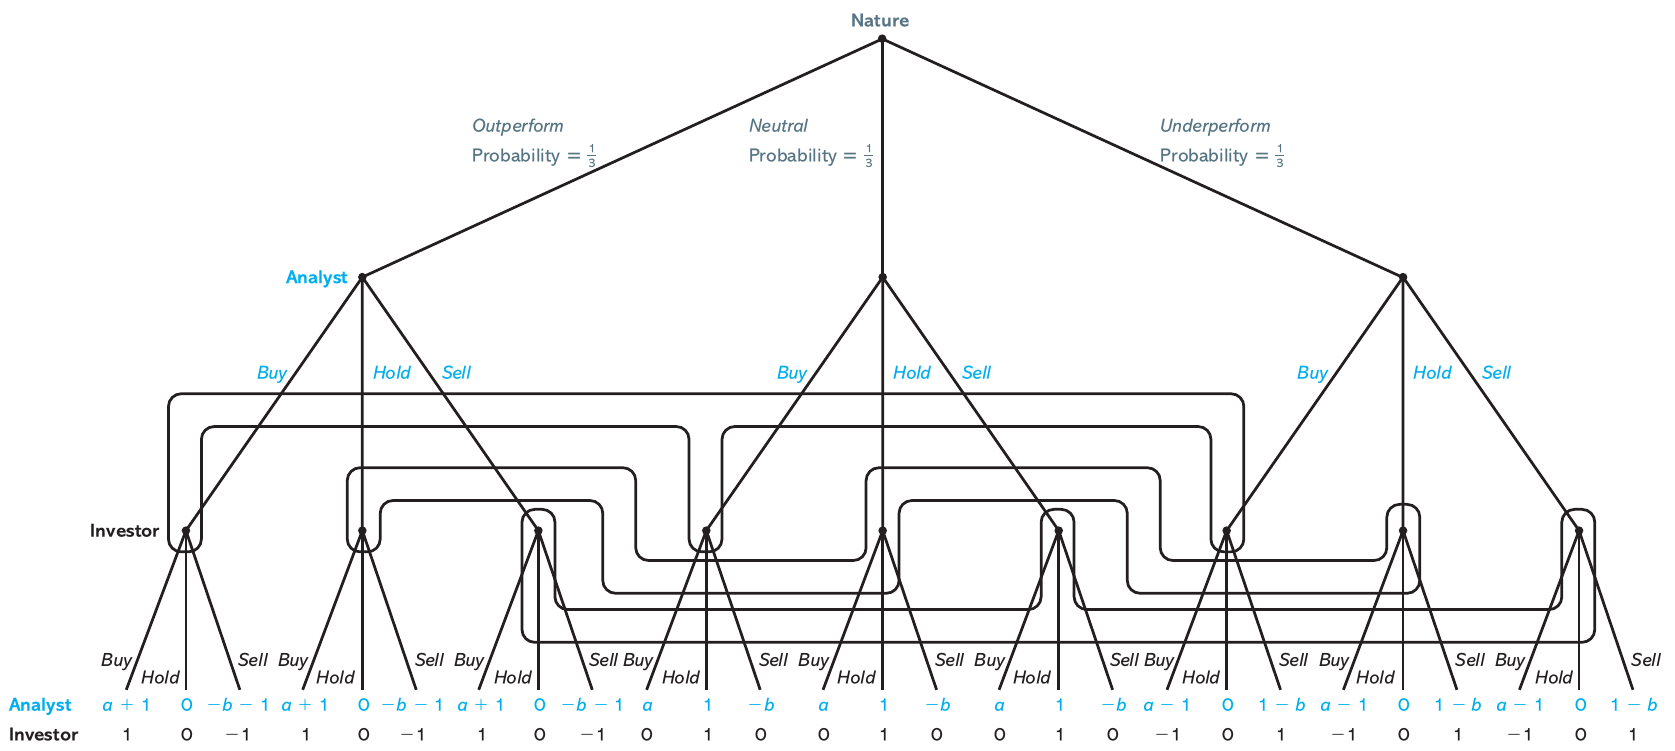
\includegraphics[width=\textwidth]{stock_cheap}
	\label{fig:figX}
\end{figure}

Para Inversor:

\begin{enumerate}
	\setlength{\itemsep}{0pt}
	\setlength{\parskip}{0pt}
	\setlength{\parsep}{0pt}
	\item Gana 1 (el máximo) siempre que la acción ejecutada corresponda con el estado de las acciones: \begin{itemize}
		\setlength{\itemsep}{0pt}
		\setlength{\parskip}{0pt}
		\setlength{\parsep}{0pt}
		\item $ \uparrow, Buy $.
		\item $ =, Hold $.
		\item $ \downarrow, Sell $.
	\end{itemize}
	\item Gana 0 con Hold si $ \uparrow , \downarrow  $, o con Buy/Sell si $ = $.
	\item Gana -1 si en $ \uparrow  $ decide vender, o si en $ \downarrow $ decide comprar. 
\end{enumerate}

Para Analista:

\begin{enumerate}
\setlength{\itemsep}{0pt}
\setlength{\parskip}{0pt}
\setlength{\parsep}{0pt}
	\item Las ganancias del analista son las mismas que las del inversor, con dos excepciones: \begin{itemize}
	\setlength{\itemsep}{0pt}
	\setlength{\parskip}{0pt}
	\setlength{\parsep}{0pt}
		\item Si el inversor compra, se suma $ a $.
		\item Si el inversor vende, se resta $ b $.
	\end{itemize}
	\item Las ganancias del analista reflejan que le va mejor cuando el portafolio del cliente tiene mejor desempeño.
	\item Notar que las ganancias no dependen del mensaje.
	\item Las cantidades $ +a, -b $ representan la disposición del analista para realizar recomendaciones de compra y de venta, respectivamente. 
\end{enumerate}

\textbf{Estrategias del analista}

Recomendar:

\begin{itemize}
	\setlength{\itemsep}{0pt}
	\setlength{\parskip}{0pt}
	\setlength{\parsep}{0pt}
	\item Buy cuando stock $ \uparrow $.
	\item Hold cuando stock $ = $.
	\item Sell cuando $ \downarrow  $.
\end{itemize}

Es decir, el analista realiza recomendaciones precisas acordes al rendimiento del stock.

\textbf{Estrategias del inversor}

Seguir la recomendación del analista.

\textbf{Creencias del inversor}

Dada la recomendación del analista, el inversor se forma las siguientes creencias:

\begin{itemize}
	\setlength{\itemsep}{0pt}
	\setlength{\parskip}{0pt}
	\setlength{\parsep}{0pt}
	\item $ p(\uparrow | Buy) = 1 $.
	\item $ p(=| Hold) = 1 $.
	\item $ p(\downarrow | Sell) = 1 $.
\end{itemize}

En este caso, es obvio que las creencias del inversor son consistentes con la estrategia del analista, y la estrategia del inversor es óptima dadas sus creencias.

Ahora, ¿qué tan óptimas son las estrategias del analista?

Suponer que el analista sabe que el stock $ \uparrow  $ (rama en extremo izquierdo), entonces su estrategia es recomendar \textbf{Buy}, lo que induce al inversor a comprar, y el analista tendrá una fanancia de $ a+1 $. Si en vez de eso hiciera una recomendación \textbf{Hold}, tendría 0, y con \textbf{Sell} de $ -b-1 $.

Ahora suponer que la verdadera calidad del stock es $ = $ (rama media). El analista tendría una ganancia de 1 si recomienda \textbf{Hold}, lo que es mejor que $ -b $.

Finalmente, suponer que el stock es $ \downarrow  $. En ese caso, la estrategia del analista le sugiere recomendar \textbf{Sell}, lo que le da una ganancia de $ 1-b $: se beneficia de dar una buena recomendación al inversor, pero obtiene un \textit{daño} por inducir la venta. Para esta misma calidad del stock, obtendría una ganancia de 0 si induce \textbf{Hold} y de $ a-1 $ si induce \textbf{Buy}.

Solo en el último caso la estrategia del analista podría ser no óptima. El equilibrio requiere que 

\begin{align*}
	\underbrace{1-b}_{\text{Sell}} &\geq \underbrace{a-1}_{\text{Buy}}\\ &\text{ y }\\
	\underbrace{1-b}_{\text{Sell}} &\geq\underbrace{0}_{\text{Hold}}
\end{align*}

Estas dos condiciones sson equivalentes a $ 1 \geq b $ y $ a+b \leq 2 $, y se resumen en $ a \leq 1, b \leq 1 $ y $a+b\leq 2 $. Si los primeros dos se cumplen, el segundo se cumple en automático.

\begin{figure}[H]
	\centering
	
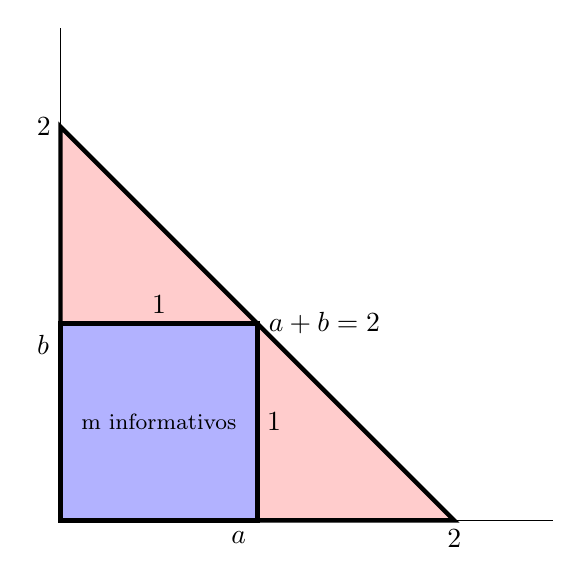
\begin{tikzpicture}[scale=2.5]
  \draw (0, 0) -- (2.5, 0);
  \draw (0, 0) -- (0, 2.5);
	\draw[ultra thick, fill=red!20](0,0)--node[below left]{$a$} (2,0)
					 	--node[right]{$a+b=2$}(0,2)
						--node[below left]{$b$}(0,0);
  \draw[ultra thick, fill = blue!30] (0, 0) rectangle (1, 1);
	\node at (0.5,0.5) {\footnotesize m informativos};
	\node[left] at (0, 2) {2};
	\node[below] at (2,0) {2};
	\node[above] at (0.5,1) {1};
	\node[right] at (1,0.5) {1};
\end{tikzpicture}
	\caption{Contenido de información de recomendaciones. El cuadrado es el área que limita los mensajes completamente informativos para los cuales, dados valores de $ a,b$ existe un equilibrio, y fuera están los mensajes parcialmente informativos.}
\end{figure}

Si el componente de inversión es muy importante, es decir, si el beneficio de inducir compra de stock es suficientemente grande ($ a>1 $) o el costo de inducir la venta de acciones es muy grande $ (b > 1) $, \textit{o ambos}, entonces no hay un equilibrio donde los mensajes (las recomendaciones) sean \textit{completamente informativas}. 

Si al analista solo le importan los intereses de su cliente, (tanto $ a ,b $ son pequeñas), un inversor puede creer en las recomendaciones.

\textbf{¿Qué pasa si $ b >1 $}

Pero si $ b>1 $ (parte superior del triángulo), entonces hay un perjuicio grande en inducir a los inversores a vender. En ese caso, ya no es un equilibrio para un analista decir la verdad \textit{completa}. ¿Puede haber un equilibrio en donde las recomendaciones sean \textit{al menos} parcialmente informativas?

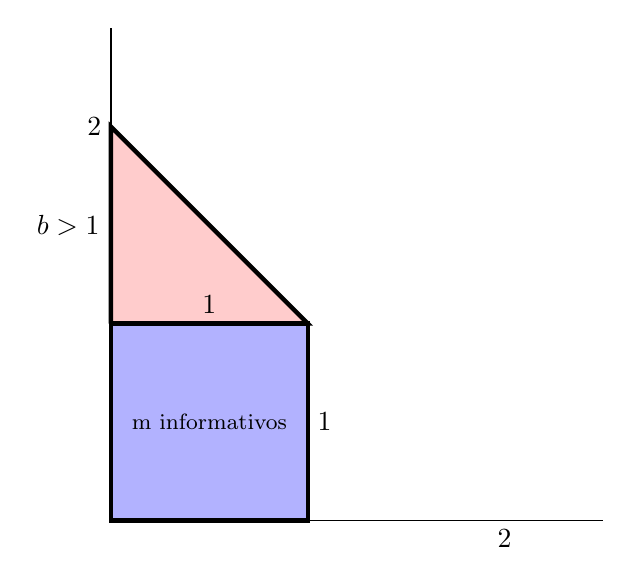
\begin{tikzpicture}[scale=2.5]
  \draw (0, 0) -- (2.5, 0);
  \draw (0, 0) -- (0, 2.5);
	\draw[ultra thick, fill=red!20] (0,1)--(1,1)--(0,2)--node[left]{$b>1$}(0,1);
  \draw[ultra thick, fill = blue!30] (0, 0) rectangle (1, 1);
	\node at (0.5,0.5) {\footnotesize m informativos};
	\node[left] at (0, 2) {2};
	\node[below] at (2,0) {2};
	\node[above] at (0.5,1) {1};
	\node[right] at (1,0.5) {1};
\end{tikzpicture}

Considerar el siguiente equilibrio \textit{semiseparador}:

\textbf{Estrategia del analista}

\begin{itemize}
\setlength{\itemsep}{0pt}
\setlength{\parskip}{0pt}
\setlength{\parsep}{0pt}
	\item \textbf{Buy} si el stock $ \uparrow , = $.
	\item \textbf{Hold} si stock $ \downarrow $
\end{itemize} 

\textbf{Estrategia del inversor}

\begin{itemize}
	\setlength{\itemsep}{0pt}
	\setlength{\parskip}{0pt}
	\setlength{\parsep}{0pt}
	\item Comprar si el analista recomienda \textbf{Buy}.
	\item Vender si el analista recomienda \textbf{Hold, Sell}.
\end{itemize}

\textbf{Creencias del inversor}

Dado que el analista recomienda Buy cuando el stock $ \uparrow, = $, el inversor debería asignar 0 a la probabilidad de $ \downarrow  $ \textit{dadas} esas recomendaciones. Dado que las probabilidades a priori para $ = $ y $ \uparrow  $ fueron de 1/3, la probabilidad posterior (la creencia actualizada del inversor) es 

\textbf{Buy:}

\begin{align*}
	p(\uparrow | Buy) &= \frac{p(Buy | \uparrow)p(\uparrow)}{p(Buy | \uparrow)p(\uparrow) + p(Buy | =)p(=) + p(Buy | \downarrow)p(\downarrow)}\\
	&\text{No consideramos } p(Buy | \downarrow) \text{ porque es }0\\
	p(\uparrow | Buy) &= \frac{\frac{1}{3}1}{\underbrace{\frac{1}{3}1}_{\text{Buy}}+\underbrace{\frac{1}{3}1}_{\text{Hold}}} = \frac{1}{2}\\ 
	&\text{Lo mismo sucede si el marcado es neutral}\\
	p(=| Buy) &= \frac{\frac{1}{3}1}{\underbrace{\frac{1}{3}1}_{\text{Hold}}+\underbrace{\frac{1}{3}1}_{\text{Buy}}} = \frac{1}{2}\\ 
	p(\downarrow | Buy) &= 0 \\ 
	&\text{dado que Buy no sucede si } \downarrow \text{ en esta estrategia}
\end{align*}

\textbf{Hold:}

\begin{align*}
	p(\uparrow | Hold) &= 0 \\
	p(= | Hold) &= 0 \\
	p(\downarrow | Hold) &= 1 \\ 
	&\text{dado que Hold sucede cuando stock tiene mal prospecto}
\end{align*}

\textbf{Sell:}

\begin{align*}
	p(\uparrow | Sell) &= \gamma_1 \\
	p(= | Sell) &= \gamma_2 \\
	p(\downarrow | Sell) &= 1-\gamma_1 - \gamma_2 
\end{align*}

Intuitivamente podemos pensar lo siguiente: si \textbf{Hold} le informa al inversor que el stock tendrá mal rendimiento, \textbf{Sell} podría informar lo mismo que \textbf{Hold} o algo \textit{peor}. Dado que esto ocurre fuera del equilibrio, las creencias del inversor están indefinidas, pero por simplicidad asumiremos $ \gamma_1 = \gamma_2 = 0 $

En resumen:

\begin{itemize}
	\setlength{\itemsep}{0pt}
	\setlength{\parskip}{0pt}
	\setlength{\parsep}{0pt}
	\item $ p(\uparrow | Buy) = 1/2 $ y $ p(= | Buy) = 1/2$.
	\item $ p(\downarrow | Hold) = p(\downarrow | Sell) = 1$.
\end{itemize}

Luego de observar la recomendación de \textbf{Buy}, las utilidades del inversor con como sigue:

\begin{align*}
	\UE{I}{\text{Buy}} = \underbrace{\frac{1}{2}1}_{\text{si stock } \uparrow} + \underbrace{\frac{1}{2}0}_{\text{si stock } =} = \frac{1}{2}
\end{align*}

Por \textbf{Hold:}

\begin{align*}
	\UE{I}{\text{Hold}} = \underbrace{\frac{1}{2}0}_{\text{si stock } \uparrow} + \underbrace{\frac{1}{2}1}_{\text{si stock } =} = \frac{1}{2}
\end{align*}

y por \textbf{Sell}:

\begin{align*}
	\UE{I}{\text{Sell}} = \underbrace{\frac{1}{2}(-1)}_{\text{si stock } \uparrow} + \underbrace{\frac{1}{2}0}_{\text{si stock } =} = -\frac{1}{2}
\end{align*}

Podemos ver que, de hecho, comprar el stock es óptimo, aunque \textit{mantener} es \textit{al menos tan bueno} como comprar. 

Si el analista recomienda \textbf{Hold, Sell} el inversor cree óptimamente que stock $ \downarrow  $, y por lo tanto vende, sin desviarse. 

¿Se desvía el analista?

Si stock $ \uparrow $ el analista obtiene $ a+1 $ si recomienda vender, y eso es mejor que inducir \textbf{Hold, Sell}, dado que en ese caso induce al inversor a vender y el analista obtiene $ -b-1 $.

Si el stock $ = $, recomienda \textbf{Buy}, en cuyo caso solo obtiene $ a $, que es mayor que $ -b $ si induce al inversor a Hold o sell.

Finalmente, si acciones $ \downarrow $ \textbf{Hold, Sell} inducen al inversor a vender, y obtiene $ 1-b $. Si por el contrario induce a comprar, obtendría $ a-1 $, por lo tanto $ 1-b \geq a-1$, o $ a+b\leq 2 $.

Siempre que $ a+b\leq 2 $ habrá un equilibrio en donde el analista recomiende Buy si stock $ \uparrow, = $ o Hold en otro caso. 

Notar que la condición $ a+b\leq 2 $ es más débil (y menos restrictiva) que la condición de equilibrio separador completo (completamente informativo), en donde además se exige $ a\leq 1, b\leq 1 $, dado que en este equilibrio $ a>1 $ o $ b>1 $ siempre que su suma sea menor a 2. POr ejemplo, se cumple si $ a=0.6 $ y $ b=1.2 $, en donde se puede perder más por inducir a inversores a vender. En este caso, un equilibrio totalmente separador e informativo no existe, pero sí existe uno semiseparador y parcialmente informativo. 

Si $ a>2 $ o $ b>2 $, los intereses del analista y el inversor divergen, y el analista está más preocupado por el impacto de las compras de stock. Esto volvería más difícil que el analista provea recomendaciones útiles a sus inversores. El contenido de información se deteriora.

\begin{figure}[H]
	\centering
	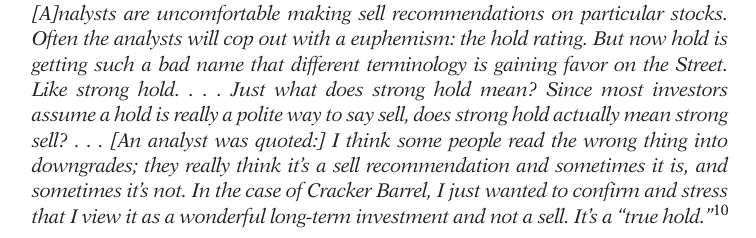
\includegraphics[width=\textwidth]{analysts.png}
\end{figure}

\end{document}